\section{Praktyczne problemy}
W tej sekcji zostaną przedstawione przypadki zastosowania teoretycznej wiedzy wraz z praktycznymi przykładami.



\subsection{Sortowanie wyników}
Czasami zdarza się, że chcemy, aby wyniki zapytania były posortowane według pewnej kolejności. Jest to oczywiście pewien dodatkowy nakład, który serwer MySQL musi wykonać podczas wykonania zapytania. W tym podrozdziale pokażę, co zrobić, aby ta operacja nie wypłyneła drastycznie na wydajność naszego zapytania.

Podstawą optymalizacji sortowania jest używanie indeksów typu B-Tree, co wynika bezpośrednio z faktu, że indeks jest posortowany względem jego kolumn. Aby przedstawić działanie indeksów na realnych przykładach przygotowałem do tego bazę StackOverflow. Z bazy usunąłem wszystkie indeksy oraz klucze główne założone na wykorzystywanych w przykładach tabelach, aby nie wpływały one na prezentowane przykłady.

MySQL może użyć indeksu do sortowania wyników w następujących przypadkach.



Najlepszym z możliwych scenariuszy wykorzystania indeksu do sortowania danych jest przypadek, kiedy kolumny użyte do sortowania odpowiadają indeksowi, a kolumny, które chcemy zwrócić jako wynik zapytania są podzbiorem kolumn indeksu.
Weźmy tabelę Users, na którą założymy indeks typu BTREE jak poniżej.

\begin{spverbatim}
	CREATE INDEX Rank_idx ON Users(Reputation, UpVotes);
\end{spverbatim}
Teraz wykonajmy zapytanie:
\begin{spverbatim}
	EXPLAIN SELECT Reputation,UpVotes FROM Users ORDER BY Reputation, UpVotes;
\end{spverbatim}
W takim przypadku poleceni EXPLAIN zwróci w kolumnie EXTRA informację: "Using index", co oznacza, że do sortowania wartości użyty został indeks znajdujący się w kolumnie key, czyli indeks, który przed chwilą stworzyliśmy.

\begin{figure}[H]
	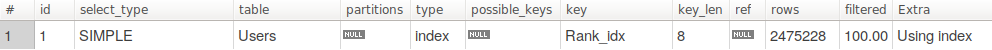
\includegraphics[scale =0.4]{explain15.png} 
\end{figure}
Jeżeli w wyniki chcemy otrzymać jedynie kolumnę \textit{Reputation}, to MySQL wciąż będzie wykorzystywał indeks do sortowania wyników, ponieważ spełnia to warunek zawierania się kolumn rezulatu zapytania w zbiorze kolumn indeksu. Sprawdźmy teraz, co się stanie jeżeli do klauzuli WHERE dodamy kolejną kolumnę:
\begin{spverbatim}
	EXPLAIN SELECT Id, Reputation, UpVotes FROM Users ORDER BY Reputation, UpVotes;
\end{spverbatim}
\begin{figure}[H]
	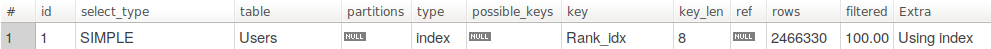
\includegraphics[scale =0.4]{explain16.png} 
\end{figure}
Widzimy, że tym razem MySQL nie wykorzystał indeksu, ale pobrał wszystkie dane i posortował wykorzystując jeden z dostępnych w MySQL algorytmów sortowania. Co ciekawe, nie zawsze musi się tak stać. MySQL na etapie analizy wykonania sprawdza, czy wydajniejsze będzie dla niego sortowanie wyników na podstawie pobranych danych, czy może, jeżeli sortujemy dane względem jednego z indeksów na tabeli, pobrać ten indeks i wykorzystać do wydajniejszego sortowania. Dodajmy teraz klucz główny dla tabeli Users i sprawdźmy, co się stanie jeżeli umieścimy go jako jedną z kolumn wyniku naszego zapytania.
\begin{spverbatim}
	ALTER TABLE Users ADD PRIMARY KEY (Id);
	EXPLAIN SELECT Id, Reputation, UpVotes FROM Users ORDER BY Reputation, UpVotes;
\end{spverbatim}

\begin{figure}[H]
	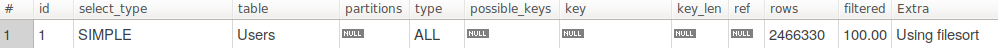
\includegraphics[scale =0.4]{explain17.png} 
\end{figure}
Wynik polecenia EXPLAIN jest interesujący. Przypomnijmy sobie zatem, w jaki sposób MySQL przechowuje dane w indeksie, jeżeli tabela posiada klucz podstawowy. W takim przypadku wiersze w liściach indeksu są identyfikowane za pomocą wartości kluczy głównych. W naszym przypadku wiersze w indeksie są identyfikowane na podstawie kolumny \textit{id}, co oznacza, że indeks zawiera wszystkie kolumny użyte w zapytaniu.

 Kolejnym często używanym zapytaniem jest pobranie wszystkich kolumn z tabeli, ale posortanie ich według określonych kolumn. Weźmy następujące zapytanie:
\begin{spverbatim}
	EXPLAIN SELECT u.* FROM Users u ORDER BY u.UpVotes, u.Reputation;
\end{spverbatim}
Tym razem MySQL znów najprawdopodobniej nie użyje indeksu do posortowania danych. Oczywiście nadal może zdecydować, że efektywniejszym będzie dodatkowe pobranie indeksu i wykorzystanie go do sortowania danych.

Przeanalizujmy teraz następne zapytanie.

\begin{spverbatim}
	EXPLAIN SELECT * FROM Users WHERE Reputation = 1 ORDER BY UpVotes;
\end{spverbatim}
\begin{figure}[H]
	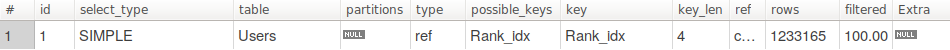
\includegraphics[scale =0.4]{explain18.png} 
\end{figure}
Tym razem MySQL znów wykorzystał indeks, do posortowania wyników. W jaki sposób to zrobił? 
Skorzystał z faktu, że indeksie są posortowane względem kolumn Reputation, a w przypadku, kiedy wartość Reputation jest równa, względem kolumny UpVote, co odpowiada wartości ORDER BY.
Sprawdźmy co się stanie, jeżeli delikatnie zmodyfikujemy zapytanie do postaci:
\begin{spverbatim}
	EXPLAIN SELECT * FROM Users WHERE Reputation > 1000 ORDER BY UpVotes;
\end{spverbatim}

W tym przypadku nie ma jednoznaczej odpowiedzi na pytanie, w jaki sposób MySQL posortuje dane. Optymalizator MySQL musi podjąć decyzję, czy warunki w klauzuli WHERE są wystarczająco selektywne, czy może pobranie indeksu i na jego podstawie przeprowadzenie sortowania będzie efektywniejsze.


